\documentclass[10pt, letterpaper]{article}

% Inhaltsverzeichnis für Pakettypen (nur für Übersicht im Header, wird nicht im Dokument angezeigt)
% 1. Seitenlayout und Ränder
% 2. Sprache und Zeichensatz
% 3. Mathematik und Theorem-Umgebungen
% 4. Eigene Makros
% 5. Diagramme und Grafiken
% 6. Tabellen und Aufzählungen
% 7. Inhaltsverzeichnis
% 8. Abschnittsüberschriften
% 9. Abstrakt-Umgebung
% 10. Todos/Notizen
% 11. Rahmen/Box-Umgebungen
% 12. Python-Integration
% 13. Literaturverwaltung
% 14. Hyperlinks
% 15. Absatzeinstellungen
% 16. Umgebungen
% 17  Graphik
% 18  Extra
% 00. Titel und Autor

% --- 1. Seitenlayout und Ränder ---
\usepackage[margin=3cm]{geometry}

% --- 2. Sprache und Zeichensatz ---
\usepackage[english]{babel}
\usepackage[T1]{fontenc}
\usepackage[utf8]{inputenc}

% --- 3. Mathematik und Theorem-Umgebungen ---
\usepackage{amsmath, amssymb, amsthm}
\usepackage{mathrsfs}
\DeclareMathOperator{\WF}{WF}

% --- 4. Eigene Makros ---
\usepackage{xcolor}
\newcommand{\SKP}{\langle\cdot,\cdot\rangle}
\newcommand{\R}{\mathbb{R}}
\newcommand{\N}{\mathbb{N}}
\newcommand{\Q}{\mathbb{Q}}
\newcommand{\Z}{\mathbb{Z}}
\newcommand{\C}{\mathbb{C}}
\newcommand{\entwurf}[1]{\textcolor{red}{#1}}

% --- 5. Diagramme und Grafiken ---
\usepackage{graphicx}
\usepackage{tikz}
\usetikzlibrary{decorations.pathreplacing, arrows.meta, positioning}
\usepackage{tikz-cd}

% --- 6. Tabellen und Aufzählungen ---
\usepackage{enumitem}
\setlist[itemize]{left=0.5cm}

\newenvironment{romanenum}[1][]
  {%
    \ifx&#1&
    \else
      \textbf{#1}\quad
    \fi
    \begin{enumerate}[label=\roman*)]
  }
  {%
    \end{enumerate}%
  }

% --- 7. Inhaltsverzeichnis ---
\usepackage{tocloft}
\renewcommand{\cftsecfont}{\footnotesize}
\renewcommand{\cftsubsecfont}{\footnotesize}
\renewcommand{\cftsubsubsecfont}{\footnotesize}
\renewcommand{\cftsecpagefont}{\footnotesize}
\renewcommand{\cftsubsecpagefont}{\footnotesize}
\renewcommand{\cftsubsubsecpagefont}{\footnotesize}
\usepackage{etoc}

% --- 8. Abschnittsüberschriften ---
\usepackage{titlesec}
\titleformat{\section}{\normalfont\large\bfseries}{\thesection}{1em}{}
\titleformat{\subsection}{\normalfont\normalsize\bfseries}{\thesubsection}{0.5em}{}
\titleformat{\subsubsection}{\normalfont\normalsize\bfseries}{\thesubsubsection}{0.5em}{}
\setcounter{secnumdepth}{4}

% --- 9. Abstrakt-Umgebung ---
\usepackage{changepage}
\renewenvironment{abstract}
  {
    \begin{adjustwidth}{1.5cm}{1.5cm}
    \small
    \textsc{Abstract. –}%
  }
  {
    \end{adjustwidth}
  }

% --- 10. Todos/Notizen ---
\usepackage{todonotes}

% --- 11. Rahmen/Box-Umgebungen ---
\usepackage{mdframed}
\usepackage{tcolorbox}
\colorlet{shadecolor}{gray!25}

\newenvironment{customTheorem}
  {\vspace{10pt}%
   \begin{mdframed}[
     backgroundcolor=gray!20,
     linewidth=0pt,
     innertopmargin=10pt,
     innerbottommargin=10pt,
     skipabove=\dimexpr\topsep+\ht\strutbox\relax,
     skipbelow=\topsep,
   ]}
  {\end{mdframed}
   \vspace{10pt}%
  }

% --- 12. Python-Integration ---
% (Deaktiviert in dieser Version, aktiviere bei Bedarf)
% \usepackage{pythontex}
% \usepackage[makestderr]{pythontex}

% --- 13. Literaturverwaltung ---
\usepackage{csquotes}
\usepackage[backend=biber, style=alphabetic, citestyle=alphabetic]{biblatex}
\addbibresource{bibliography.bib}

% --- 14. Hyperlinks ---
\usepackage{hyperref}
\hypersetup{
  colorlinks   = true,
  urlcolor     = blue,
  linkcolor    = blue,
  citecolor    = blue,
  frenchlinks  = true
}

% --- 15. Absatzeinstellungen ---
\usepackage[parfill]{parskip}
\sloppy

% --- 16. Umgebungen ---
\usepackage{thmtools}

\newcommand{\CustomHeading}[3]{%
  \par\medskip\noindent%
  \textbf{#1 #2} \textnormal{(#3)}.\enskip%
}

\newenvironment{DEF}[2]{\begin{unitbox}\CustomHeading{Definition}{#1}{#2}}{\end{unitbox}}
\newenvironment{PROP}[2]{\begin{unitbox}\CustomHeading{Proposition}{#1}{#2}}{\end{unitbox}}
\newenvironment{THEO}[2]{\begin{unitbox}\CustomHeading{Theorem}{#1}{#2}}{\end{unitbox}}
\newenvironment{LEM}[2]{\begin{unitbox}\CustomHeading{Lemma}{#1}{#2}}{\end{unitbox}}
\newenvironment{KORO}[2]{\begin{unitbox}\CustomHeading{Corollar}{#1}{#2}}{\end{unitbox}}
\newenvironment{REM}[2]{\begin{unitbox}\CustomHeading{Remark}{#1}{#2}}{\end{unitbox}}
\newenvironment{EXA}[2]{\begin{unitbox}\CustomHeading{Example}{#1}{#2}}{\end{unitbox}}
\newenvironment{STUD}[2]{\begin{unitbox}\CustomHeading{Study}{#1}{#2}}{\end{unitbox}}
\newenvironment{CONC}[2]{\begin{unitbox}\CustomHeading{Concept}{#1}{#2}}{\end{unitbox}}
\newenvironment{OTH}[2]{\begin{unitbox}\CustomHeading{Other}{#1}{#2}}{\end{unitbox}}
\newenvironment{EXE}[2]{\begin{unitbox}\CustomHeading{Exercise}{#1}{#2}}{\end{unitbox}}
\newenvironment{MOT}[2]{\begin{unitbox}\CustomHeading{Motivation}{#1}{#2}}{\end{unitbox}}
\newenvironment{PROOF}[2]{\begin{unitbox}\CustomHeading{Proof}{#1}{#2}}{\end{unitbox}}

% --- Unit Umgebung für Source-Inhalte ---
\usepackage{mdframed}
\newmdenv[
  linewidth=1pt,
  topline=false,
  bottomline=false,
  rightline=false,
  leftmargin=0cm,
  rightmargin=0cm,
  skipabove=10pt,
  skipbelow=10pt,
  innertopmargin=0.5\baselineskip,
  innerbottommargin=0.5\baselineskip,
  backgroundcolor=gray!10,
  linecolor=gray
]{unitbox}

\newenvironment{unit}[1]
  {\begin{unitbox}\textbf{Unit #1}\par\smallskip}
  {\end{unitbox}}

% --- 17. Graphik ---
\usepackage{graphicx}
\graphicspath{ {./images/} }
\usepackage[export]{adjustbox}

% --- 18. Extras ---
\usepackage{stmaryrd}
\usepackage{bbold}  % falls du athbb{1} nutzen willst

% --- 00. Titel und Autor ---
\title{Mein Titel}
\author{Tim Jaschik}
\date{\today}

\begin{document}

\maketitle
\rule{\textwidth}{0.5pt}
\begin{abstract}
Kurze Beschreibung …
\end{abstract}
\rule{\textwidth}{0.5pt}
\vspace{0.5cm}

\tableofcontents

\pagebreak


\section*{Chapter 12 Tensors}

Much of the technology of smooth manifold theory is designed to allow the concepts of linear algebra to be applied to smooth manifolds. Calculus tells us how to approximate smooth objects by linear ones, and the abstract definitions of manifold theory give a way to interpret these linear approximations in a coordinate-independent way.

In this chapter we carry this idea much further, by generalizing from linear maps to multilinear ones-those that take several vectors as input and depend linearly on each one separately. Although linear maps are paramount in differential geometry, there are many situations in which multilinear maps play important geometric roles. We will introduce a unified language for talking about multilinear maps: the language of tensors. This leads to the concepts of tensors and tensor fields on manifolds.

We begin with tensors on a vector space, which are multilinear generalizations of covectors; a covector is the special case of a tensor of rank one. We give two alternative definitions of tensors on a vector space: on the one hand, they are elements of the abstract "tensor product" of the dual vector space with itself; on the other hand, they are real-valued multilinear functions of several vectors. Each definition is useful in certain contexts. We deal primarily with covariant tensors, but we also give a brief introduction to contravariant tensors and tensors of mixed variance.

Next we introduce two special classes of tensors: the symmetric tensors, whose values are unchanged by permutations of their arguments, and the alternating tensors, whose values change sign when two argument are interchanged.

We then move to smooth manifolds, where we define tensor fields and tensor bundles. After describing the coordinate representations of tensor fields, we describe how they can be pulled back by smooth maps. We also show how the Lie derivative operator can be extended to tensors: the Lie derivative of a tensor field with respect to a vector field is a measure of the rate of change of the tensor field along the flow of the vector field.

Tensors will pervade the rest of the book, and we will see significant applications of them when we study Riemannian metrics, differential forms, orientations, integration, de Rham cohomology, foliations, and symplectic structures.

\section*{Multilinear Algebra}
We have seen some of the important roles played in manifold theory by covectors, which are real-valued linear functions on a vector space. In their simplest form, tensors are just real-valued multilinear functions of one or more variables; simple examples include covectors, inner products, and determinants. To set the stage for our study of tensors, in this section we develop some of the basic properties of multilinear functions in a general setting.

\begin{DEF}{GA-L13-02-01}{Multilineare Abbildung}
Suppose $V_{1}, \ldots, V_{k}$, and $W$ are vector spaces. A map $F: V_{1} \times \cdots \times V_{k} \rightarrow W$ is said to be multilinear if it is linear as a function of each variable separately when the others are held fixed: for each $i$,\\
$F\left(v_{1}, \ldots, a v_{i}+a^{\prime} v_{i}^{\prime}, \ldots, v_{k}\right)=a F\left(v_{1}, \ldots, v_{i}, \ldots, v_{k}\right)+a^{\prime} F\left(v_{1}, \ldots, v_{i}^{\prime}, \ldots, v_{k}\right)$.

(A multilinear function of one variable is just a linear function, and a multilinear function of two variables is generally called bilinear.) Let us write $\mathrm{L}\left(V_{1}, \ldots, V_{k} ; W\right)$ for the set of all multilinear maps from $V_{1} \times \cdots \times V_{k}$ to $W$. It is a vector space under the usual operations of pointwise addition and scalar multiplication:
$$
\begin{aligned}
\left(F+F^{\prime}\right)\left(v_{1}, \ldots, v_{k}\right) & =F\left(v_{1}, \ldots, v_{k}\right)+F^{\prime}\left(v_{1}, \ldots, v_{k}\right) \\
(a F)\left(v_{1}, \ldots, v_{k}\right) & =a\left(F\left(v_{1}, \ldots, v_{k}\right)\right)
\end{aligned}
$$
\end{DEF}





Here are a few examples to keep in mind.



\section*{Example 12.1 (Some Familiar Multilinear Functions).}


\begin{EXA}{GA-L13-02-02}{Dot-Produkt}
The dot product in $\mathbb{R}^{n}$ is a scalar-valued bilinear function of two vectors, used to compute lengths of vectors and angles between them.
\end{EXA}




\begin{EXA}{GA-L13-02-03}{Kreuzprodukt}
The cross product in $\mathbb{R}^{3}$ is a vector-valued bilinear function of two vectors, used to compute areas of parallelograms and to find a third vector orthogonal to two given ones.
\end{EXA}




\begin{EXA}{GA-L13-02-04}{Determinante}
The determinant is a real-valued multilinear function of $n$ vectors in $\mathbb{R}^{n}$, used to detect linear independence and to compute the volume of the parallelepiped spanned by the vectors.
\end{EXA}



\begin{EXA}{GA-L13-02-05}{Lie-Klammer}
The bracket in a Lie algebra g is a g -valued bilinear function of two elements of g .
\end{EXA}


The next example is probably not as familiar, but it is extremely important.


Example 12.2 (Tensor Products of Covectors). 

\begin{EXA}{GA-L13-02-06}{Tensor Produkt für Kovektoren}
Suppose $V$ is a vector space, and $\omega, \eta \in V^{*}$. Define a function $\omega \otimes \eta: V \times V \rightarrow \mathbb{R}$ by
$$
\omega \otimes \eta\left(v_{1}, v_{2}\right)=\omega\left(v_{1}\right) \eta\left(v_{2}\right)
$$
where the product on the right is just ordinary multiplication of real numbers. The linearity of $\omega$ and $\eta$ guarantees that $\omega \otimes \eta$ is a bilinear function of $v_{1}$ and $v_{2}$, so it is an element of $\mathrm{L}(V, V ; \mathbb{R})$. For example, if ( $e^{1}, e^{2}$ ) denotes the standard dual basis for $\left(\mathbb{R}^{2}\right)^{*}$, then $e^{1} \otimes e^{2}: \mathbb{R}^{2} \times \mathbb{R}^{2} \rightarrow \mathbb{R}$ is the bilinear function
$$
e^{1} \otimes e^{2}((w, x),(y, z))=w z
$$
\end{EXA}



\begin{EXA}{GA-L13-02-07}{Tensor Produkt für Multilineare Abbildungen}
The last example can be generalized to arbitrary real-valued multilinear functions as follows: let $V_{1}, \ldots, V_{k}, W_{1}, \ldots, W_{l}$ be real vector spaces, and suppose $F \in \mathrm{~L}\left(V_{1}, \ldots, V_{k} ; \mathbb{R}\right)$ and $G \in \mathrm{~L}\left(W_{1}, \ldots, W_{l} ; \mathbb{R}\right)$. Define a function
$$
F \otimes G: V_{1} \times \cdots \times V_{k} \times W_{1} \times \cdots \times W_{l} \rightarrow \mathbb{R}
$$
by
$$
F \otimes G\left(v_{1}, \ldots, v_{k}, w_{1}, \ldots, w_{l}\right)=F\left(v_{1}, \ldots, v_{k}\right) G\left(w_{1}, \ldots, w_{l}\right)
$$
It follows from the multilinearity of $F$ and $G$ that $F \otimes G\left(v_{1}, \ldots, v_{k}, w_{1}, \ldots, w_{l}\right)$ depends linearly on each argument $v_{i}$ or $w_{j}$ separately, so $F \otimes G$ is an element of $\mathrm{L}\left(V_{1}, \ldots, V_{k}, W_{1}, \ldots, W_{l} ; \mathbb{R}\right)$, called the tensor product of $\boldsymbol{F}$ and $\boldsymbol{G}$.
\end{EXA}



\begin{itemize}
  \item Exercise 12.3. Show that the tensor product operation is bilinear and associative:\\
  $F \otimes G$ depends bilinearly on $F$ and $G$, and $(F \otimes G) \otimes H=F \otimes(G \otimes H)$.\\
\end{itemize}


\begin{PROP}{GA-L13-02-08}{Tensor Produkt für Multilineare Abbildungen ist bilinear und assoziativ}
1. Bilinearität: Das Tensorprodukt $F \otimes G$ hängt bilinear von den beiden Faktoren $F$ und $G$ ab. Das heißt, die Abbildung
$$
(F, G) \mapsto F \otimes G
$$
ist linear in jedem der beiden Argumente, wenn das jeweils andere festgehalten wird. Formal bedeutet das:
$$
\begin{aligned}
\left(\lambda_1 F_1+\lambda_2 F_2\right) \otimes G & =\lambda_1\left(F_1 \otimes G\right)+\lambda_2\left(F_2 \otimes G\right), \\
F \otimes\left(\mu_1 G_1+\mu_2 G_2\right) & =\mu_1\left(F \otimes G_1\right)+\mu_2\left(F \otimes G_2\right),
\end{aligned}
$$
für beliebige Skalare $\lambda_1, \lambda_2, \mu_1, \mu_2$ und beliebige Vektoren (bzw. Tensoren) $F_1, F_2, G_1, G_2$.

2. Assoziativität: Das Tensorprodukt ist assoziativ, d. h. für beliebige Tensoren $F, G, H$ gilt:
$$
(F \otimes G) \otimes H=F \otimes(G \otimes H)
$$
wobei beide Seiten kanonisch als Elemente eines dreifachen Tensorprodukts identifiziert werden. Es gibt also einen natürlichen Isomorphismus
$$
(V \otimes W) \otimes U \cong V \otimes(W \otimes U)
$$
für Vektorräume $V, W, U$, und unter dieser Identifikation stimmen die beiden Tensorprodukte überein.
\end{PROP}



\begin{REM}{GA-L13-02-09}{Notation des Tensorprodukts}
Because of the result of the preceding exercise, we can write tensor products of three or more multilinear functions unambiguously without parentheses. If $F_{1}, \ldots, F_{l}$ are multilinear functions depending on $k_{1}, \ldots, k_{l}$ variables, respectively, their tensor product $F_{1} \otimes \cdots \otimes F_{l}$ is a multilinear function of $k=k_{1}+\cdots+k_{l}$ variables, whose action on $k$ vectors is given by inserting the first $k_{1}$ vectors into $F_{1}$, the next $k_{2}$ vectors into $F_{2}$, and so forth, and multiplying the results together. For example, if $F$ and $G$ are multilinear functions of two vectors and $H$ is a multilinear function of three, then
$$
F \otimes G \otimes H\left(v_{1}, \ldots, v_{7}\right)=F\left(v_{1}, v_{2}\right) G\left(v_{3}, v_{4}\right) H\left(v_{5}, v_{6}, v_{7}\right)
$$
If $\omega^{j} \in V_{j}^{*}$ for $j=1, \ldots, k$, then $\omega^{1} \otimes \cdots \otimes \omega^{k} \in \mathrm{~L}\left(V_{1}, \ldots, V_{k} ; \mathbb{R}\right)$ is the multilinear function given by
$$
\omega^{1} \otimes \cdots \otimes \omega^{k}\left(v_{1}, \ldots, v_{k}\right)=\omega^{1}\left(v_{1}\right) \cdots \omega^{k}\left(v_{k}\right)
$$
\end{REM}



The tensor product operation is important in part because of its role in the following proposition. The notation in this proposition is ugly because of the profusion of indices, but the underlying idea is simple: a basis for any space of multilinear functions can be formed by taking all possible tensor products of basis covectors.


Proposition 12.4 (A Basis for the Space of Multilinear Functions). 


\begin{PROP}{GA-L13-02-10}{Basis für den Raum der multilinearen Abbildungen}
Let $V_{1}, \ldots, V_{k}$ be real vector spaces of dimensions $n_{1}, \ldots, n_{k}$, respectively. For each $j \in\{1, \ldots, k\}$, let $\left(E_{1}^{(j)}, \ldots, E_{n_{j}}^{(j)}\right)$ be a basis for $V_{j}$, and let $\left(\varepsilon_{(j)}^{1}, \ldots, \varepsilon_{(j)}^{n_{j}}\right)$ be the corresponding dual basis for $V_{j}^{*}$. Then the set
$$
\mathcal{B}=\left\{\varepsilon_{(1)}^{i_{1}} \otimes \cdots \otimes \varepsilon_{(k)}^{i_{k}}: 1 \leq i_{1} \leq n_{1}, \ldots, 1 \leq i_{k} \leq n_{k}\right\}
$$
is a basis for $\mathrm{L}\left(V_{1}, \ldots, V_{k} ; \mathbb{R}\right)$, which therefore has dimension equal to $n_{1} \cdots n_{k}$.
\end{PROP}


Proof. 



\begin{PROOF}{GA-L13-02-11}{P: Basis für den Raum der multilinearen Abbildungen}
We need to show that $\mathscr{B}$ is linearly independent and spans $\mathrm{L}\left(V_{1}, \ldots, V_{k} ; \mathbb{R}\right)$. Suppose $F \in \mathrm{~L}\left(V_{1}, \ldots, V_{k} ; \mathbb{R}\right)$ is arbitrary. For each ordered $k$-tuple $\left(i_{1}, \ldots, i_{k}\right)$ of\\
integers with $1 \leq i_{j} \leq n_{j}$, define a number $F_{i_{1} \ldots i_{k}}$ by
$
F_{i_{1} \ldots i_{k}}=F\left(E_{i_{1}}^{(1)}, \ldots, E_{i_{k}}^{(k)}\right)
$
We will show that
$
F=F_{i_{1} \ldots i_{k}} \varepsilon_{(1)}^{i_{1}} \otimes \cdots \otimes \varepsilon_{(k)}^{i_{k}}
$
(with the summation convention in effect as usual), from which it follows that $\mathscr{B}$ spans $\mathrm{L}\left(V_{1}, \ldots, V_{k} ; \mathbb{R}\right)$. For any $k$-tuple of vectors $\left(v_{1}, \ldots, v_{k}\right) \in V_{1} \times \cdots \times V_{k}$, write $v_{1}=v_{1}^{i_{1}} E_{i_{1}}^{(1)}, \ldots, v_{k}=v_{k}^{i_{k}} E_{i_{k}}^{(k)}$, and compute
$
\begin{aligned}
F_{i_{1} \ldots i_{k}} \varepsilon_{(1)}^{i_{1}} \otimes \cdots \otimes \varepsilon_{(k)}^{i_{k}}\left(v_{1}, \ldots, v_{k}\right) & =F_{i_{1} \ldots i_{k}} \varepsilon_{(1)}^{i_{1}}\left(v_{1}\right) \cdots \varepsilon_{(k)}^{i_{k}}\left(v_{k}\right) \\
& =F_{i_{1} \ldots i_{k}} v_{1}^{i_{1}} \cdots v_{k}^{i_{k}}
\end{aligned}
$
while $F\left(v_{1}, \ldots, v_{k}\right)$ is equal to the same thing by multilinearity. This proves the claim.

To show that $\mathscr{B}$ is linearly independent, suppose some linear combination equals zero:
$
F_{i_{1} \ldots i_{k}} \varepsilon_{(1)}^{i_{1}} \otimes \cdots \otimes \varepsilon_{(k)}^{i_{k}}=0
$
Apply this to any ordered $k$-tuple of basis vectors, $\left(E_{j_{1}}^{(1)}, \ldots, E_{j_{k}}^{(k)}\right)$. By the same computation as above, this implies that each coefficient $F_{j_{1} \ldots j_{k}}$ is zero. Thus, the only linear combination of elements of $\mathscr{B}$ that sums to zero is the trivial one.
\end{PROOF}




\begin{CONC}{GA-L13-02-12}{Komponenten von multilinearen Abbildungen durch Anwendung auf Basisvektoren}
This proof shows, by the way, that the components $F_{i_{1} \ldots i_{k}}$ of a multilinear function $F$ in terms of the basis elements in $\mathscr{B}$ are given by
$$F_{i_1 \ldots i_k}=F\left(E_{i_1}^{(1)}, \ldots, E_{i_k}^{(k)}\right)$$
Thus, $F$ is completely determined by its action on all possible sequences of basis vectors.
\end{CONC}



\section*{Abstract Tensor Products of Vector Spaces}


\begin{REM}{GA-L13-02-13}{Konkreter und Abstrakter Zugang zu Tensorprodukt}
The results of the previous section showed that the vector space of multilinear functions $\mathrm{L}\left(V_{1}, \ldots, V_{k} ; \mathbb{R}\right)$ can be viewed as the set of all linear combinations of objects of the form $\omega^{1} \otimes \cdots \otimes \omega^{k}$, where $\omega^{1}, \ldots, \omega^{k}$ are covectors. 

In this section, we give a construction that makes sense of such linear combinations of tensor products in a more abstract setting. The construction is a bit involved, but the idea is simple: given finite-dimensional vector spaces $V_{1}, \ldots, V_{k}$, we will construct a new vector space $V_{1} \otimes \cdots \otimes V_{k}$ whose dimension is the product of the dimensions of the $V_{i}$ 's, and which consists of "formal linear combinations" of objects of the form $v_{1} \otimes \cdots \otimes v_{k}$ for $v_{i} \in V_{i}$, defined in such a way that $v_{1} \otimes \cdots \otimes v_{k}$ depends linearly on each $v_{i}$ separately. (Many of the concepts we introduce in this section-at least the parts that do not refer explicitly to finite bases-work equally well in the infinite-dimensional case; but we mostly restrict our attention to the finite-dimensional case in order to keep things simple.)
\end{REM}

\begin{DEF}{GA-L13-02-14}{Formale Linearkombination und freier Vektorraum}
To begin, we need to make sense of "formal linear combinations." Let $S$ be a set. Roughly speaking, a formal linear combination of elements of $S$ is an expression of the form $\sum_{i=1}^{m} a_{i} x_{i}$, where $a_{1}, \ldots, a_{m}$ are real numbers and $x_{1}, \ldots, x_{m}$ are elements of $S$. 
Of course, since we are not assuming that $S$ has any algebraic structure, we cannot literally add elements of $S$ together or multiply them by numbers. But the essential feature of such an expression is that it is completely determined by which elements of $S$ appear in the sum, and what coefficients appear with them. 

Thus, we make the following definition: for any set $S$, a formal linear combination of elements of $\boldsymbol{S}$ is a function $f: S \rightarrow \mathbb{R}$ such that $f(s)=0$ for all but finitely many $s \in S$. The free (real) vector space on $S$, denoted by $\mathcal{F}(S)$, is the set of all formal linear combinations of elements of $S$. Under pointwise addition and scalar multiplication, $\mathcal{F}(S)$ becomes a vector space over $\mathbb{R}$.

For each element $x \in S$, there is a function $\delta_{x} \in \mathscr{F}(S)$ that takes the value 1 on $x$ and zero on all other elements of $S$; typically we identify this function with $x$ itself, and thus think of $S$ as a subset of $\mathscr{F}(S)$. Every element $f \in \mathscr{F}(S)$ can then be written uniquely in the form $f=\sum_{i=1}^{m} a_{i} x_{i}$, where $x_{1}, \ldots, x_{m}$ are the elements of $S$ for which $f\left(x_{i}\right) \neq 0$, and $a_{i}=f\left(x_{i}\right)$. Thus, $S$ is a basis for $\mathscr{F}(S)$, which is therefore finite-dimensional if and only if $S$ is a finite set.
\end{DEF}

Proposition 12.5 (Characteristic Property of the Free Vector Space). 


\begin{PROP}{GA-L13-02-15}{Erweiterung von Abbildung von Basismenge in Vektorraum für freie Vektorräume}
For any set $S$ and any vector space $W$, every map $A: S \rightarrow W$ has a unique extension to a linear map $\bar{A}: \mathcal{F}(S) \rightarrow W$.
\end{PROP}

\begin{itemize}
  \item Exercise 12.6. Prove the preceding proposition.
\end{itemize}


\begin{DEF}{GA-L13-02-16}{Abstrakte Tensorprodukt via freie Vektorräume}
Now let $V_{1}, \ldots, V_{k}$ be real vector spaces. We begin by forming the free vector space $\mathscr{F}\left(V_{1} \times \cdots \times V_{k}\right)$, which is the set of all finite formal linear combinations of $k$-tuples ( $v_{1}, \ldots, v_{k}$ ) with $v_{i} \in V_{i}$ for $i=1, \ldots, k$. Let $\mathcal{R}$ be the subspace of $\mathcal{F}\left(V_{1} \times \cdots \times V_{k}\right)$ spanned by all elements of the following forms:
$$
\begin{gathered}
\left(v_{1}, \ldots, a v_{i}, \ldots, v_{k}\right)-a\left(v_{1}, \ldots, v_{i}, \ldots, v_{k}\right), \\
\left(v_{1}, \ldots, v_{i}+v_{i}^{\prime}, \ldots, v_{k}\right)-\left(v_{1}, \ldots, v_{i}, \ldots, v_{k}\right)-\left(v_{1}, \ldots, v_{i}^{\prime}, \ldots, v_{k}\right),
\end{gathered}
$$
with $v_{j}, v_{j}^{\prime} \in V_{j}, i \in\{1, \ldots, k\}$, and $a \in \mathbb{R}$.\\
Define the tensor product of the spaces $V_{1}, \ldots, V_{k}$, denoted by $V_{1} \otimes \cdots \otimes V_{k}$, to be the following quotient vector space:
$$
V_{1} \otimes \cdots \otimes V_{k}=\mathscr{F}\left(V_{1} \times \cdots \times V_{k}\right) / \mathscr{R},
$$
and let $\Pi: \mathcal{F}\left(V_{1} \times \cdots \times V_{k}\right) \rightarrow V_{1} \otimes \cdots \otimes V_{k}$ be the natural projection. The equivalence class of an element $\left(v_{1}, \ldots, v_{k}\right)$ in $V_{1} \otimes \cdots \otimes V_{k}$ is denoted by
$$
v_{1} \otimes \cdots \otimes v_{k}=\Pi\left(v_{1}, \ldots, v_{k}\right),
$$
and is called the (abstract) tensor product of $\boldsymbol{v}_{\mathbf{1}}, \ldots, \boldsymbol{v}_{\boldsymbol{k}}$.
\end{DEF}


\begin{REM}{GA-L13-02-17}{Eigenschaften des abstrakten Tensorprodukts}
It follows from the definition that abstract tensor products satisfy
$$
\begin{aligned}
v_{1} \otimes \cdots \otimes a v_{i} \otimes \cdots \otimes v_{k}= & a\left(v_{1} \otimes \cdots \otimes v_{i} \otimes \cdots \otimes v_{k}\right), \\
v_{1} \otimes \cdots \otimes\left(v_{i}+v_{i}^{\prime}\right) \otimes \cdots \otimes v_{k}= & \left(v_{1} \otimes \cdots \otimes v_{i} \otimes \cdots \otimes v_{k}\right) \\
& +\left(v_{1} \otimes \cdots \otimes v_{i}^{\prime} \otimes \cdots \otimes v_{k}\right) .
\end{aligned}
$$
\end{REM}


\begin{REM}{GA-L13-02-18}{todo abstrakte tensorprodukt}
Note that the definition implies that every element of $V_{1} \otimes \cdots \otimes V_{k}$ can be expressed as a linear combination of elements of the form $v_{1} \otimes \cdots \otimes v_{k}$ for $v_{i} \in V_{i}$; but it is not true in general that every element of the tensor product space is of the form $v_{1} \otimes \cdots \otimes v_{k}$ (see Problem 12-1).
\end{REM}

Proposition 12.7 (Characteristic Property of the Tensor Product Space). 


\begin{PROP}{GA-L13-02-19}{Charakteristische Eigenschaften des Tensor Produkt Raumes}
Let $V_{1}, \ldots, V_{k}$ be finite-dimensional real vector spaces. If $A: V_{1} \times \cdots \times V_{k} \rightarrow X$ is any multilinear map into a vector space $X$, then there is a unique linear map $\tilde{A}: V_{1} \otimes \cdots \otimes V_{k} \rightarrow X$ such that the following diagram commutes:\\
\[
\begin{tikzcd}[row sep=large, column sep=large]
V_1 \times \cdots \times V_k \arrow[r, "A"] \arrow[d, "\pi"'] & X \\
V_1 \otimes \cdots \otimes V_k \arrow[ru, dashed, "\widetilde{A}"']
\end{tikzcd}
\]
where $\pi$ is the map $\pi\left(v_{1}, \ldots, v_{k}\right)=v_{1} \otimes \cdots \otimes v_{k}$.
\end{PROP}


Proof. 


\begin{PROOF}{GA-L13-02-20}{P: Charakteristische Eigenschaften des Tensor Produkt Raumes}
First note that any map $A: V_{1} \times \cdots \times V_{k} \rightarrow X$ extends uniquely to a linear map $\bar{A}: \mathcal{F}\left(V_{1} \times \cdots \times V_{k}\right) \rightarrow X$ by the characteristic property of the free vector space. This map is characterized by the fact that $\bar{A}\left(v_{1}, \ldots, v_{k}\right)=A\left(v_{1}, \ldots, v_{k}\right)$ whenever $\left(v_{1}, \ldots, v_{k}\right) \in V_{1} \times \cdots \times V_{k} \subseteq \mathscr{F}\left(V_{1} \times \cdots \times V_{k}\right)$. The fact that $A$ is multilinear means precisely that the subspace $\mathcal{R}$ is contained in the kernel of $\bar{A}$, because
$$
\begin{aligned}
\bar{A}\left(v_{1}, \ldots, a v_{i}, \ldots, v_{k}\right) & =A\left(v_{1}, \ldots, a v_{i}, \ldots, v_{k}\right)=a A\left(v_{1}, \ldots, v_{i}, \ldots, v_{k}\right) \\
& =a \bar{A}\left(v_{1}, \ldots, v_{i}, \ldots, v_{k}\right)=\bar{A}\left(a\left(v_{1}, \ldots, v_{i}, \ldots, v_{k}\right)\right)
\end{aligned}
$$
with a similar computation for the other expression in (12.4). Therefore, $\bar{A}$ descends to a linear map $\tilde{A}: V_{1} \otimes \cdots \otimes V_{k}=\mathscr{F}\left(V_{1} \times \cdots \times V_{k}\right) / \mathcal{R} \rightarrow X$ satisfying $\tilde{A} \circ \Pi=\bar{A}$. Since $\pi$ is equal to the inclusion $V_{1} \times \cdots \times V_{k} \hookrightarrow \mathscr{F}\left(V_{1} \times \cdots \times V_{k}\right)$ followed by $\Pi$, this implies $\tilde{A} \circ \pi=A$, which is (12.6). Uniqueness follows from the fact that every element of $V_{1} \otimes \cdots \otimes V_{k}$ can be written as a linear combination of elements of the form $v_{1} \otimes \cdots \otimes v_{k}$, and $\tilde{A}$ is uniquely determined on such elements by
$$
\tilde{A}\left(v_{1} \otimes \cdots \otimes v_{k}\right)=\bar{A}\left(v_{1}, \ldots, v_{k}\right)=A\left(v_{1}, \ldots, v_{k}\right)
$$
\end{PROOF}



The reason this is called the characteristic property is that it uniquely characterizes the tensor product up to isomorphism; see Problem 12-3.



The next result is an analogue of Proposition 12.4 for abstract tensor product spaces.

Proposition 12.8 (A Basis for the Tensor Product Space). 


\begin{PROP}{GA-L13-02-21}{Basis für den Tensor Produkt Raum}
Suppose $V_{1}, \ldots, V_{k}$ are real vector spaces of dimensions $n_{1}, \ldots, n_{k}$, respectively. For each $j=1, \ldots, k$, suppose $\left(E_{1}^{(j)}, \ldots, E_{n_{j}}^{(j)}\right)$ is a basis for $V_{j}$. Then the set
$$
\mathcal{C}=\left\{E_{i_{1}}^{(1)} \otimes \cdots \otimes E_{i_{k}}^{(k)}: 1 \leq i_{1} \leq n_{1}, \ldots, 1 \leq i_{k} \leq n_{k}\right\}
$$
is a basis for $V_{1} \otimes \cdots \otimes V_{k}$, which therefore has dimension equal to $n_{1} \cdots n_{k}$.
\end{PROP}



Proof. 


\begin{PROOF}{GA-L13-02-22}{P: Basis für den Tensor Produkt Raum}
Elements of the form $v_{1} \otimes \cdots \otimes v_{k}$ span the tensor product space by definition; expanding each $v_{i}$ in such an expression in terms of its basis representation shows that $\mathcal{C}$ spans $V_{1} \otimes \cdots \otimes V_{k}$.

To prove that $\mathcal{C}$ is linearly independent, assume that some linear combination of elements of $\mathscr{C}$ is equal to zero:

$$
a^{i_{1} \ldots i_{k}} E_{i_{1}}^{(1)} \otimes \cdots \otimes E_{i_{k}}^{(k)}=0
$$

For each ordered $k$-tuple of indices ( $m_{1}, \ldots, m_{k}$ ), define a multilinear function $\tau^{m_{1} \ldots m_{k}}: V_{1} \times \cdots \times V_{k} \rightarrow \mathbb{R}$ by

$$
\tau^{m_{1} \ldots m_{k}}\left(v_{1}, \ldots, v_{k}\right)=\varepsilon_{(1)}^{m_{1}}\left(v_{1}\right) \cdots \varepsilon_{(k)}^{m_{k}}\left(v_{k}\right)
$$

where $\left(\varepsilon_{(j)}^{i}\right)$ is the basis for $V_{j}^{*}$ dual to $\left(E_{i}^{(j)}\right)$. Because $\tau^{m_{1} \ldots m_{k}}$ is multilinear, it descends to a linear function $\widetilde{\tau}^{m_{1} \ldots m_{k}}: V_{1} \otimes \cdots \otimes V_{k} \rightarrow \mathbb{R}$ by the characteristic property of the tensor product. It follows that

$$
\begin{aligned}
0 & =\tilde{\tau}^{m_{1} \ldots m_{k}}\left(a^{i_{1} \ldots i_{k}} E_{i_{1}}^{(1)} \otimes \cdots \otimes E_{i_{k}}^{(k)}\right) \\
& =a^{i_{1} \ldots i_{k}} \tau^{m_{1} \ldots m_{k}}\left(E_{i_{1}}^{(1)}, \ldots, E_{i_{k}}^{(k)}\right)=a^{m_{1} \ldots m_{k}}
\end{aligned}
$$

which shows that $\mathscr{C}$ is linearly independent.
\end{PROOF}




Proposition 12.9 (Associativity of Tensor Product Spaces). 



\begin{PROP}{GA-L13-02-23}{Assoziativität von Tensor Produkt Raum}
Let $V_{1}, V_{2}, V_{3}$ be finite-dimensional real vector spaces. There are unique isomorphisms
$$
V_{1} \otimes\left(V_{2} \otimes V_{3}\right) \cong V_{1} \otimes V_{2} \otimes V_{3} \cong\left(V_{1} \otimes V_{2}\right) \otimes V_{3}
$$
under which elements of the forms $v_{1} \otimes\left(v_{2} \otimes v_{3}\right), v_{1} \otimes v_{2} \otimes v_{3}$, and $\left(v_{1} \otimes v_{2}\right) \otimes v_{3}$ all correspond.
\end{PROP}



Proof. 

\begin{PROOF}{GA-L13-02-24}{P: Assoziativität von Tensor Produkt Raum}
We construct the isomorphism $V_{1} \otimes V_{2} \otimes V_{3} \cong\left(V_{1} \otimes V_{2}\right) \otimes V_{3}$; the other one is constructed similarly. The map $\alpha: V_{1} \times V_{2} \times V_{3} \rightarrow\left(V_{1} \otimes V_{2}\right) \otimes V_{3}$ defined by
$$
\alpha\left(v_{1}, v_{2}, v_{3}\right)=\left(v_{1} \otimes v_{2}\right) \otimes v_{3}
$$
is obviously multilinear, and thus by the characteristic property of the tensor product it descends uniquely to a linear map $\widetilde{\alpha}: V_{1} \otimes V_{2} \otimes V_{3} \rightarrow\left(V_{1} \otimes V_{2}\right) \otimes V_{3}$ satisfying $\widetilde{\alpha}\left(v_{1} \otimes v_{2} \otimes v_{3}\right)=\left(v_{1} \otimes v_{2}\right) \otimes v_{3}$ for all $v_{1} \in V_{1}, v_{2} \in V_{2}$, and $v_{3} \in V_{3}$. Because $\left(V_{1} \otimes V_{2}\right) \otimes V_{3}$ is spanned by elements of the form $\left(v_{1} \otimes v_{2}\right) \otimes v_{3}, \tilde{\alpha}$ is surjective, and therefore it is an isomorphism for dimensional reasons. It is clearly the unique such isomorphism, because any other would have to agree with $\tilde{\alpha}$ on the set of all elements of the form $v_{1} \otimes v_{2} \otimes v_{3}$, which spans $V_{1} \otimes V_{2} \otimes V_{3}$.
\end{PROOF}


The connection between tensor products in this abstract setting and the more concrete tensor products of multilinear functionals that we defined earlier is based on the following proposition.

Proposition 12.10 (Abstract vs. Concrete Tensor Products). 

\begin{PROP}{GA-L13-02-25}{Beziehung zwischen abstraktem undkKonkretem Tensor Produkt}
If $V_{1}, \ldots, V_{k}$ are finite-dimensional vector spaces, there is a canonical isomorphism
$$
V_{1}^{*} \otimes \cdots \otimes V_{k}^{*} \cong \mathrm{~L}\left(V_{1}, \ldots, V_{k} ; \mathbb{R}\right)
$$
under which the abstract tensor product defined by 
$$v_1 \otimes \cdots \otimes v_k=\Pi\left(v_1, \ldots, v_k\right)$$
corresponds to the tensor product of covectors defined by
$$\omega^1 \otimes \cdots \otimes \omega^k\left(v_1, \ldots, v_k\right)=\omega^1\left(v_1\right) \cdots \omega^k\left(v_k\right)$$
The connection between tensor products in this abstract setting and the more concrete tensor products of multilinear functionals that we defined earlier is based on the following proposition.
\end{PROP}


Proof. 

\begin{PROOF}{GA-L13-02-26}{P: Beziehung zwischen abstraktem undkKonkretem Tensor Produkt}
First, define a map $\Phi: V_{1}^{*} \times \cdots \times V_{k}^{*} \rightarrow \mathrm{~L}\left(V_{1}, \ldots, V_{k} ; \mathbb{R}\right)$ by
$$
\Phi\left(\omega^{1}, \ldots, \omega^{k}\right)\left(v_{1}, \ldots, v_{k}\right)=\omega^{1}\left(v_{1}\right) \cdots \omega^{k}\left(v_{k}\right)
$$
(There is no implied summation in this formula.) The expression on the right depends linearly on each $v_{i}$, so $\Phi\left(\omega^{1}, \ldots, \omega^{k}\right)$ is indeed an element of the space $\mathrm{L}\left(V_{1}, \ldots, V_{k} ; \mathbb{R}\right)$. It is easy to check that $\Phi$ is multilinear as a function of $\omega^{1}, \ldots, \omega^{k}$, so by the characteristic property it descends uniquely to a linear map $\widetilde{\Phi}$ from $V_{1}^{*} \otimes \cdots \otimes V_{k}^{*}$ to $\mathrm{L}\left(V_{1}, \ldots, V_{k} ; \mathbb{R}\right)$, which satisfies
$$
\widetilde{\Phi}\left(\omega^{1} \otimes \cdots \otimes \omega^{k}\right)\left(v_{1}, \ldots, v_{k}\right)=\omega^{1}\left(v_{1}\right) \cdots \omega^{k}\left(v_{k}\right)
$$
It follows immediately from the definition that $\widetilde{\Phi}$ takes abstract tensor products to tensor products of covectors. It also takes the basis of $V_{1}^{*} \otimes \cdots \otimes V_{k}^{*}$ given by Proposition 12.8 to the basis for $\mathrm{L}\left(V_{1}, \ldots, V_{k} ; \mathbb{R}\right)$ of Proposition 12.4, so it is an isomorphism. (Although we used bases to prove that $\widetilde{\Phi}$ is an isomorphism, $\widetilde{\Phi}$ itself is canonically defined without reference to any basis.)
\end{PROOF}


\begin{CONC}{GA-L13-02-27}{Verwendung des Isomorphismus zwischen abstraktem Tensor Produkt Raum und Vektorraum der Multilinearabbildungen}
Using this canonical isomorphism, we henceforth use the notation $V_{1}^{*} \otimes \cdots \otimes V_{k}^{*}$ to denote either the abstract tensor product space or the space $\mathrm{L}\left(V_{1}, \ldots, V_{k} ; \mathbb{R}\right)$, focusing on whichever interpretation is more convenient for the problem at hand.
\end{CONC}


\begin{CONC}{GA-L13-02-28}{Verwendung der Identifikation von Vektorraum mit dem zweiten dualen Vektorraum für end. dim. Vektorräume}
Since we are assuming the vector spaces are all finite-dimensional, we can also identify each $V_{j}$ with its second dual space $V_{j}^{* *}$, and thereby obtain another canonical identification
$$
V_{1} \otimes \cdots \otimes V_{k} \cong \mathrm{~L}\left(V_{1}^{*}, \ldots, V_{k}^{*} ; \mathbb{R}\right)
$$
\end{CONC}



\pagebreak



\section*{Covariant and Contravariant Tensors on a Vector Space}



\begin{DEF}{GA-L13-03-01}{Kovarianter k-Tensor auf Vektorräumen}
Let $V$ be a finite-dimensional real vector space. If $k$ is a positive integer, a covariant $\boldsymbol{k}$-tensor on $\boldsymbol{V}$ is an element of the $k$-fold tensor product $V^{*} \otimes \cdots \otimes V^{*}$, which we typically think of as a real-valued multilinear function of $k$ elements of $V$ :
$$
\alpha: \underbrace{V \times \cdots \times V}_{k \text { copies }} \rightarrow \mathbb{R}
$$
The number $k$ is called the rank of $\boldsymbol{\alpha}$. A 0-tensor is, by convention, just a real number (a real-valued function depending multilinearly on no vectors!). We denote the vector space of all covariant $k$-tensors on $V$ by the shorthand notation
$$
T^{k}\left(V^{*}\right)=\underbrace{V^{*} \otimes \cdots \otimes V^{*}}_{k \text { copies }}
$$
\end{DEF}



Let us look at some examples.


Example 12.11 (Covariant Tensors). 

\begin{EXA}{GA-L13-03-02}{Lineare Funktionale als korvariante 1-Tensoren}
Let $V$ be a finite-dimensional vector space. Every linear functional $\omega: V \rightarrow \mathbb{R}$ is multilinear, so a covariant 1-tensor is just a covector. Thus, $T^{1}\left(V^{*}\right)$ is equal to $V^{*}$.
\end{EXA}


\begin{EXA}{GA-L13-03-03}{Reell-wertige Bilinearabbildung als kovariante 2 Tensoren}
Let $V$ be a finite-dimensional vector space. A covariant 2-tensor on $V$ is a real-valued bilinear function of two vectors, also called a bilinear form. One example is the dot product on $\mathbb{R}^{n}$. More generally, every inner product is a covariant 2-tensor.
\end{EXA}


\begin{EXA}{GA-L13-03-04}{Determinante als kovarianter k-Tensor}
Let $V$ be a finite-dimensional vector space. The determinant, thought of as a function of $n$ vectors, is a covariant $n$-tensor on $\mathbb{R}^{n}$.
\end{EXA}



For some purposes, it is important to generalize the notion of covariant tensors as follows. 


\begin{DEF}{GA-L13-03-05}{Kontravarianter k-Tensor auf Vektorräumen}
For any finite-dimensional real vector space $V$, we define the space of contravariant tensors on $\boldsymbol{V}$ of rank $\boldsymbol{k}$ to be the vector space
$$
T^{k}(V)=\underbrace{V \otimes \cdots \otimes V}_{k \text { copies }}
$$
In particular, $T^{1}(V)=V$, and by convention $T^{0}(V)=\mathbb{R}$. Because we are assuming that $V$ is finite-dimensional, it is possible to identify this space with the set of multilinear functionals of $k$ covectors:
$$
T^{k}(V) \cong\{\text { multilinear functions } \alpha: \underbrace{V^{*} \times \cdots \times V^{*}}_{k \text { copies }} \rightarrow \mathbb{R}\}
$$
But for most purposes, it is easier to think of contravariant tensors simply as elements of the abstract tensor product space.
\end{DEF}


\begin{DEF}{GA-L13-03-06}{k,l-Tensor auf Vektorräumen}
Even more generally, for any nonnegative integers $k, l$, we define the space of mixed tensors on V of type ( $k, l$ ) as
$$
T^{(k, l)}(V)=\underbrace{V \otimes \cdots \otimes V}_{k \text { copies }} \otimes \underbrace{V^{*} \otimes \cdots \otimes V^{*}}_{l \text { copies }}
$$

Some of these spaces are identical:
$$
\begin{aligned}
& T^{(0,0)}(V)=T^{0}\left(V^{*}\right)=T^{0}(V)=\mathbb{R}, \\
& T^{(0,1)}(V)=T^{1}\left(V^{*}\right)=V^{*}, \\
& T^{(1,0)}(V)=T^{1}(V)=V, \\
& T^{(0, k)}(V)=T^{k}\left(V^{*}\right), \\
& T^{(k, 0)}(V)=T^{k}(V) .
\end{aligned}
$$
\end{DEF}

(Be aware that the notation $T^{(k, l)}(V)$ is not universal. Another notation that is in common use for this space is $T_{l}^{k}(V)$. To make matters worse, some books reverse the roles of $k$ and $l$ in either of these notations; for example, the previous edition of this text used the notation $T_{k}^{l}(V)$ for the space we are here denoting by $T^{(k, l)}(V)$.

We have chosen the notation given here because it is common and nearly always means the same thing. The moral, as usual, is that when you read any differential geometry book, you need to make sure you understand the author's notational conventions.)

\begin{REM}{GA-L13-03-07}{Basis für Tensor Räume}
When $V$ is finite-dimensional, any choice of basis for $V$ automatically yields bases for all of the tensor spaces over $V$. The following corollary follows immediately from Proposition 12.8.
\end{REM}


Corollary 12.12. 

\begin{KORO}{GA-L13-03-08}{Basis für Tensor Räume aus (duale) Basis von Vektorraum }
Let $V$ be an $n$-dimensional real vector space. Suppose ( $E_{i}$ ) is any basis for $V$ and $\left(\varepsilon^{j}\right)$ is the dual basis for $V^{*}$. Then the following sets constitute bases for the tensor spaces over $V$ :
$$
\begin{gathered}
\left\{\varepsilon^{i_{1}} \otimes \cdots \otimes \varepsilon^{i_{k}}: 1 \leq i_{1}, \ldots, i_{k} \leq n\right\} \quad \text { for } T^{k}\left(V^{*}\right) ; \\
\left\{E_{i_{1}} \otimes \cdots \otimes E_{i_{k}}: 1 \leq i_{1}, \ldots, i_{k} \leq n\right\} \quad \text { for } T^{k}(V) ; \\
\left\{E_{i_{1}} \otimes \cdots \otimes E_{i_{k}} \otimes \varepsilon^{j_{1}} \otimes \cdots \otimes \varepsilon^{j_{l}}: 1 \leq i_{1}, \ldots, i_{k}, j_{1}, \ldots, j_{l} \leq n\right\} \quad \text { for } T^{(k, l)}(V) .
\end{gathered}
$$
Therefore, $\operatorname{dim} T^{k}\left(V^{*}\right)=\operatorname{dim} T^{k}(V)=n^{k}$ and $\operatorname{dim} T^{(k, l)}(V)=n^{k+l}$.\\
In particular, once a basis is chosen for $V$, every covariant $k$-tensor $\alpha \in T^{k}\left(V^{*}\right)$ can be written uniquely in the form
$$
\alpha=\alpha_{i_{1} \ldots i_{k}} \varepsilon^{i_{1}} \otimes \cdots \otimes \varepsilon^{i_{k}},
$$
where the $n^{k}$ coefficients $\alpha_{i_{1} \ldots i_{k}}$ are determined by
$$
\alpha_{i_{1} \ldots i_{k}}=\alpha\left(E_{i_{1}}, \ldots, E_{i_{k}}\right) .
$$
\end{KORO}


\begin{EXA}{GA-L13-03-09}{Darstellung der Bilinearformen}
For example, $T^{2}\left(V^{*}\right)$ is the space of bilinear forms on $V$, and every bilinear form can be written as $\beta=\beta_{i j} \varepsilon^{i} \otimes \varepsilon^{j}$ for some uniquely determined $n \times n$ matrix ( $\beta_{i j}$ ).
\end{EXA}

In this book we are concerned primarily with covariant tensors. Thus tensors will always be understood to be covariant unless we explicitly specify otherwise. However, it is important to be aware that contravariant and mixed tensors play important roles in more advanced parts of differential geometry, especially Riemannian geometry.


\pagebreak


\section*{Symmetric and Alternating Tensors}
In general, rearranging the arguments of a covariant tensor need not have any predictable effect on its value. However, some special tensors-the dot product, for example-do not change their values when their arguments are rearranged. Others-notably the determinant-change sign whenever two arguments are interchanged. In this section, we describe two classes of tensors that change in a simple way when their arguments are rearranged: the symmetric ones and the alternating ones.

\section*{Symmetric Tensors}
Let $V$ be a finite-dimensional vector space. A covariant $k$-tensor $\alpha$ on $V$ is said to be symmetric if its value is unchanged by interchanging any pair of arguments:

$$
\alpha\left(v_{1}, \ldots, v_{i}, \ldots, v_{j}, \ldots, v_{k}\right)=\alpha\left(v_{1}, \ldots, v_{j}, \ldots, v_{i}, \ldots, v_{k}\right)
$$

whenever $1 \leq i<j \leq k$.

\begin{itemize}
  \item Exercise 12.13. Show that the following are equivalent for a covariant $k$-tensor $\alpha$ :\\
(a) $\alpha$ is symmetric.\\
(b) For any vectors $v_{1}, \ldots, v_{k} \in V$, the value of $\alpha\left(v_{1}, \ldots, v_{k}\right)$ is unchanged when $v_{1}, \ldots, v_{k}$ are rearranged in any order.\\
(c) The components $\alpha_{i_{1} \ldots i_{k}}$ of $\alpha$ with respect to any basis are unchanged by any permutation of the indices.
\end{itemize}

The set of symmetric covariant $k$-tensors is a linear subspace of the space $T^{k}\left(V^{*}\right)$ of all covariant $k$-tensors on $V$; we denote this subspace by $\Sigma^{k}\left(V^{*}\right)$. There is a natural projection from $T^{k}\left(V^{*}\right)$ to $\Sigma^{k}\left(V^{*}\right)$ defined as follows. First, let $S_{k}$ denote the symmetric group on k elements, that is, the group of permutations of the set $\{1, \ldots, k\}$. Given a $k$-tensor $\alpha$ and a permutation $\sigma \in S_{k}$, we define a new $k$-tensor ${ }^{\sigma} \alpha$ by

$$
{ }^{\sigma} \alpha\left(v_{1}, \ldots, v_{k}\right)=\alpha\left(v_{\sigma(1)}, \ldots, v_{\sigma(k)}\right) .
$$

Note that ${ }^{\tau}\left({ }^{\sigma} \alpha\right)={ }^{\tau \sigma} \alpha$, where $\tau \sigma$ represents the composition of $\tau$ and $\sigma$, that is, $\tau \sigma(i)=\tau(\sigma(i))$. (This is the reason for putting $\sigma$ before $\alpha$ in the notation ${ }^{\sigma} \alpha$, instead of after it.) We define a projection Sym: $T^{k}\left(V^{*}\right) \rightarrow \Sigma^{k}\left(V^{*}\right)$ called symmetrization by

$$
\operatorname{Sym} \alpha=\frac{1}{k!} \sum_{\sigma \in S_{k}}{ }^{\sigma} \alpha .
$$

More explicitly, this means that

$$
(\operatorname{Sym} \alpha)\left(v_{1}, \ldots, v_{k}\right)=\frac{1}{k!} \sum_{\sigma \in S_{k}} \alpha\left(v_{\sigma(1)}, \ldots, v_{\sigma(k)}\right) .
$$

Proposition 12.14 (Properties of Symmetrization). Let $\alpha$ be a covariant tensor on a finite-dimensional vector space.\\
(a) Sym $\alpha$ is symmetric.\\
(b) Sym $\alpha=\alpha$ if and only if $\alpha$ is symmetric.

Proof. Suppose $\alpha \in T^{k}\left(V^{*}\right)$. If $\tau \in S_{k}$ is any permutation, then

$$
\begin{aligned}
(\operatorname{Sym} \alpha)\left(v_{\tau(1)}, \ldots, v_{\tau(k)}\right) & =\frac{1}{k!} \sum_{\sigma \in S_{k}}{ }^{\sigma} \alpha\left(v_{\tau(1)}, \ldots, v_{\tau(k)}\right) \\
& =\frac{1}{k!} \sum_{\sigma \in S_{k}}{ }^{\tau \sigma} \alpha\left(v_{1}, \ldots, v_{k}\right)
\end{aligned}
$$

$$
\begin{aligned}
& =\frac{1}{k!} \sum_{\eta \in S_{k}}{ }^{\eta} \alpha\left(v_{1}, \ldots, v_{k}\right) \\
& =(\operatorname{Sym} \alpha)\left(v_{1}, \ldots, v_{k}\right)
\end{aligned}
$$

where we have substituted $\eta=\tau \sigma$ in the second-to-last line and used the fact that $\eta$ runs over all of $S_{k}$ as $\sigma$ does. This shows that Sym $\alpha$ is symmetric.

If $\alpha$ is symmetric, then it follows from Exercise 12.13(b) that ${ }^{\sigma} \alpha=\alpha$ for every $\sigma \in S_{k}$, so it follows immediately that Sym $\alpha=\alpha$. On the other hand, if Sym $\alpha=\alpha$, then $\alpha$ is symmetric because part (a) shows that $\operatorname{Sym} \alpha$ is.

If $\alpha$ and $\beta$ are symmetric tensors on $V$, then $\alpha \otimes \beta$ is not symmetric in general. However, using the symmetrization operator, it is possible to define a new product that takes a pair of symmetric tensors and yields another symmetric tensor. If $\alpha \in$ $\Sigma^{k}\left(V^{*}\right)$ and $\beta \in \Sigma^{l}\left(V^{*}\right)$, we define their symmetric product to be the ( $k+l$ )tensor $\alpha \beta$ (denoted by juxtaposition with no intervening product symbol) given by

$$
\alpha \beta=\operatorname{Sym}(\alpha \otimes \beta) .
$$

More explicitly, the action of $\alpha \beta$ on vectors $v_{1}, \ldots, v_{k+l}$ is given by

$$
\alpha \beta\left(v_{1}, \ldots, v_{k+l}\right)=\frac{1}{(k+l)!} \sum_{\sigma \in S_{k+l}} \alpha\left(v_{\sigma(1)}, \ldots, v_{\sigma(k)}\right) \beta\left(v_{\sigma(k+1)}, \ldots, v_{\sigma(k+l)}\right) .
$$

\section*{Proposition 12.15 (Properties of the Symmetric Product).}
(a) The symmetric product is symmetric and bilinear: for all symmetric tensors $\alpha$, $\beta, \gamma$ and all $a, b \in \mathbb{R}$,

$$
\begin{aligned}
\alpha \beta & =\beta \alpha \\
(a \alpha+b \beta) \gamma & =a \alpha \gamma+b \beta \gamma=\gamma(a \alpha+b \beta)
\end{aligned}
$$

(b) If $\alpha$ and $\beta$ are covectors, then

$$
\alpha \beta=\frac{1}{2}(\alpha \otimes \beta+\beta \otimes \alpha)
$$

\begin{itemize}
  \item Exercise 12.16. Prove Proposition 12.15.
\end{itemize}

\section*{Alternating Tensors}
We continue to assume that $V$ is a finite-dimensional real vector space. A covariant $k$-tensor $\alpha$ on $V$ is said to be alternating (or antisymmetric or skew-symmetric) if it changes sign whenever two of its arguments are interchanged. This means that for all vectors $v_{1}, \ldots, v_{k} \in V$ and every pair of distinct indices $i, j$ it satisfies

$$
\alpha\left(v_{1}, \ldots, v_{i}, \ldots, v_{j}, \ldots, v_{k}\right)=-\alpha\left(v_{1}, \ldots, v_{j}, \ldots, v_{i}, \ldots, v_{k}\right) .
$$

Alternating covariant $k$-tensors are also variously called exterior forms, multicovectors, or $\boldsymbol{k}$-covectors. The subspace of all alternating covariant $k$-tensors on $V$ is denoted by $\Lambda^{k}\left(V^{*}\right) \subseteq T^{k}\left(V^{*}\right)$.

Recall that for any permutation $\sigma \in S_{k}$, the sign of $\sigma$, denoted by sgn $\sigma$, is equal to +1 if $\sigma$ is even (i.e., can be written as a composition of an even number of transpositions), and -1 if $\sigma$ is odd (see Proposition B.26). The following exercise is an analogue of Exercise 12.13.

\begin{itemize}
  \item Exercise 12.17. Show that the following are equivalent for a covariant $k$-tensor $\alpha$ :\\
(a) $\alpha$ is alternating.\\
(b) For any vectors $v_{1}, \ldots, v_{k}$ and any permutation $\sigma \in S_{k}$,
\end{itemize}

$$
\alpha\left(v_{\sigma(1)}, \ldots, v_{\sigma(k)}\right)=(\operatorname{sgn} \sigma) \alpha\left(v_{1}, \ldots, v_{k}\right) .
$$

(c) With respect to any basis, the components $\alpha_{i_{1} \ldots i_{k}}$ of $\alpha$ change sign whenever two indices are interchanged.

Every 0-tensor (which is just a real number) is both symmetric and alternating, because there are no arguments to interchange. Similarly, every 1-tensor is both symmetric and alternating. An alternating 2-tensor on $V$ is a skew-symmetric bilinear form. It is interesting to note that every covariant 2-tensor $\beta$ can be expressed as a sum of an alternating tensor and a symmetric one, because

$$
\begin{aligned}
\beta(v, w) & =\frac{1}{2}(\beta(v, w)-\beta(w, v))+\frac{1}{2}(\beta(v, w)+\beta(w, v)) \\
& =\alpha(v, w)+\sigma(v, w),
\end{aligned}
$$

where $\alpha(v, w)=\frac{1}{2}(\beta(v, w)-\beta(w, v))$ is an alternating tensor, and $\sigma(v, w)=$ $\frac{1}{2}(\beta(v, w)+\beta(w, v))$ is symmetric. This is not true for tensors of higher rank, as Problem 12-7 shows.

There are analogues of symmetrization and symmetric products that apply to alternating tensors, but we will put off introducing them until Chapter 14, where we will study the properties of alternating tensors in much more detail.



\pagebreak


\section*{Tensors and Tensor Fields on Manifolds}


\begin{DEF}{GA-L13-04-01}{k,l-Tensorbündel auf Mannigfaltigkeit}
Let $M$ be a smooth manifold with or without boundary. We define the bundle of covariant $\boldsymbol{k}$-tensors on $\boldsymbol{M}$ by
$$
T^{k} T^{*} M=\coprod_{p \in M} T^{k}\left(T_{p}^{*} M\right)
$$
Analogously, we define the bundle of contravariant $\boldsymbol{k}$-tensors by
$$
T^{k} T M=\coprod_{p \in M} T^{k}\left(T_{p} M\right)
$$
and the bundle of mixed tensors of type ( $\boldsymbol{k}, \boldsymbol{l}$ ) by
$$
T^{(k, l)} T M=\coprod_{p \in M} T^{(k, l)}\left(T_{p} M\right) .
$$

There are natural identifications
$$
\begin{aligned}
& T^{(0,0)} T M=T^{0} T^{*} M=T^{0} T M=M \times \mathbb{R}, \\
& T^{(0,1)} T M=T^{1} T^{*} M=T^{*} M, \\
& T^{(1,0)} T M=T^{1} T M=T M, \\
& T^{(0, k)} T M=T^{k} T^{*} M, \\
& T^{(k, 0)} T M=T^{k} T M .
\end{aligned}
$$
Any one of these bundles is called a tensor bundle over M. (Thus, the tangent and cotangent bundles are special cases of tensor bundles.)
\end{DEF}


\begin{DEF}{GA-L13-04-02}{k,l-Tensorfelder in Tensorbündeln}
A section of a tensor bundle is called a (covariant, contravariant, or mixed) tensor field on M. A smooth tensor field is a section that is smooth in the usual sense of smooth sections of vector bundles. Using the identifications above, we see that contravariant 1-tensor fields are the same as vector fields, and covariant 1 -tensor fields are covector fields. Because a 0-tensor is just a real number, a 0-tensor field is the same as a continuous real-valued function.

The spaces of smooth sections of these tensor bundles, $\Gamma\left(T^{k} T^{*} M\right), \Gamma\left(T^{k} T M\right)$, and $\Gamma\left(T^{(k, l)} T M\right)$, are infinite-dimensional vector spaces over $\mathbb{R}$, and modules over $C^{\infty}(M)$.
\end{DEF}


\begin{DEF}{GA-L13-04-03}{k,l-Tensorfelder in lokalen Koordinaten}
In any smooth local coordinates $\left(x^{i}\right)$, sections of these bundles can be written (using the summation convention) as
$$
A= \begin{cases}A_{i_{1} \ldots i_{k}} d x^{i_{1}} \otimes \cdots \otimes d x^{i_{k}}, & A \in \Gamma\left(T^{k} T^{*} M\right) \\ A^{i_{1} \ldots i_{k}} \frac{\partial}{\partial x^{i_{1}}} \otimes \cdots \otimes \frac{\partial}{\partial x^{i_{k}}}, & A \in \Gamma\left(T^{k} T M\right) \\ A_{j_{1} \ldots l_{l}}^{i_{1} \ldots i_{k}} \frac{\partial}{\partial x^{i_{1}}} \otimes \cdots \otimes \frac{\partial}{\partial x^{i_{k}}} \otimes d x^{j_{1}} \otimes \cdots \otimes d x^{j_{l}}, & A \in \Gamma\left(T^{(k, l)} T M\right)\end{cases}
$$
The functions $A_{i_{1} \ldots i_{k}}, A^{i_{1} \ldots i_{k}}$, or $A_{j_{1} \ldots i_{l}}^{i_{1} \ldots i_{k}}$ are called the component functions of $\boldsymbol{A}$ in the chosen coordinates.
\end{DEF} 

Because smooth covariant tensor fields occupy most of our attention, we adopt the following shorthand notation for the space of all smooth covariant $k$-tensor fields:
$$
\mathcal{T}^{k}(M)=\Gamma\left(T^{k} T^{*} M\right)
$$


Proposition 12.19 (Smoothness Criteria for Tensor Fields). 


\begin{PROP}{GA-L13-04-04}{Glatteis-Kriterium für Tensorfelder}
Let $M$ be a smooth manifold with or without boundary, and let $A: M \rightarrow T^{(0, k)} T M$ be a rough section. The following are equivalent.
\begin{itemize}
  \item[(a)] $A$ is smooth.
  \item[(b)] In every smooth coordinate chart, the component functions of $A$ are smooth.
  \item[(c)] Each point of $M$ is contained in some coordinate chart in which $A$ has smooth component functions.
  \item[(d)] If $X_1, \ldots, X_k \in \mathfrak{X}(M)$, then the function 
  \[
  A(X_1, \ldots, X_k)(p) = A_p(X_1|_p, \ldots, X_k|_p)
  \]
  is smooth on $M$.
  \item[(e)] Whenever $X_1, \ldots, X_k$ are smooth vector fields defined on some open subset $U \subseteq M$, the function $A(X_1, \ldots, X_k)$ is smooth on $U$.
\end{itemize}
\end{PROP}


\begin{itemize}
  \item Exercise 12.20. Prove Proposition 12.19.
  \item Exercise 12.21. Formulate and prove smoothness criteria analogous to those of Proposition 12.19 for contravariant and mixed tensor fields.
\end{itemize}

Proposition 12.22. 

\begin{PROP}{GA-L13-04-05}{Glattheit und Komponentenformeln für $f A$ und $A \otimes B$}
Suppose $M$ is a smooth manifold with or without boundary, $A \in T^{(0, k)} T M, B \in T^{(0, k)} T M$, and $f \in C^{\infty}(M)$. Then $f A$ and $A \otimes B$ are also smooth tensor fields, whose components in any smooth local coordinate chart are
$$
\begin{aligned}
(f A)_{i_{1} \ldots i_{k}} & =f A_{i_{1} \ldots i_{k}} \\
(A \otimes B)_{i_{1} \ldots i_{k+l}} & =A_{i_{1} \ldots i_{k}} B_{i_{k+1} \ldots i_{k+l}}
\end{aligned}
$$
\end{PROP}

Exercise 12.23. Prove Proposition 12.22.\\



\begin{CONC}{GA-L13-04-08}{Kommentar zu Tensor Charakterisierungs Lemma}
Proposition 12.19(d): If $X_1, \ldots, X_k \in \mathfrak{X}(M)$, then the function 
  \[
  A(X_1, \ldots, X_k)(p) = A_p(X_1|_p, \ldots, X_k|_p)
  \]
is smooth on $M$, shows that if $A$ is a smooth covariant $k$-tensor field on $M$ and $X_{1}, \ldots, X_{k}$ are smooth vector fields, then $A\left(X_{1}, \ldots, X_{k}\right)$ is a smooth realvalued function on $M$. Thus $A$ induces a map

$$
\underbrace{\mathfrak{X}(M) \times \cdots \times \mathfrak{X}(M)}_{k \text { copies }} \rightarrow C^{\infty}(M) .
$$

It is easy to see that this map is multilinear over $\mathbb{R}$. In fact, more is true: it is multilinear over $\boldsymbol{C}^{\infty}(\boldsymbol{M})$, which means that for $f, f^{\prime} \in C^{\infty}(M)$ and $X_{i}, X_{i}^{\prime} \in$ $\mathfrak{X}(M)$, we have

$$
\begin{aligned}
& A\left(X_{1}, \ldots, f X_{i}+f^{\prime} X_{i}^{\prime}, \ldots, X_{k}\right) \\
& \quad=f A\left(X_{1}, \ldots, X_{i}, \ldots, X_{k}\right)+f^{\prime} A\left(X_{1}, \ldots, X_{i}^{\prime}, \ldots, X_{k}\right)
\end{aligned}
$$

This property turns out to be characteristic of smooth tensor fields, as the next lemma shows.
\end{CONC}


Lemma 12.24 (Tensor Characterization Lemma). 



\begin{LEM}{GA-L13-04-06}{Tensor Charakterisierungs Lemma}
A map
$$
\mathcal{A}: \underbrace{\mathfrak{X}(M) \times \cdots \times \mathfrak{X}(M)}_{k \text { copies }} \rightarrow C^{\infty}(M)
$$
is induced by a smooth covariant $k$-tensor field as above if and only if it is multilinear over $C^{\infty}(M)$.
\end{LEM}

Proof. 


\begin{PROOF}{GA-L13-04-07}{P: Tensor Charakterisierungs Lemma}
We already noted that if $A$ is a smooth covariant $k$-tensor field, then the map $\left(X_{1}, \ldots, X_{k}\right) \mapsto A\left(X_{1}, \ldots, X_{k}\right)$ is multilinear over $C^{\infty}(M)$. To prove the converse,\\
we proceed as in the proof of the bundle homomorphism characterization lemma (Lemma 10.29).

Suppose, therefore, that $\mathscr{A}$ is a map as in (12.7), and assume that $\mathscr{A}$ is multilinear over $C^{\infty}(M)$. We show first that $\mathscr{A}$ acts locally. If $X_{i}$ is a smooth vector field that vanishes on a neighborhood $U$ of $p$, we can choose a bump function $\psi$ supported in $U$ such that $\psi(p)=1$; then because $\psi X_{i} \equiv 0$ we have
$$
0=\mathscr{A}\left(X_{1}, \ldots, \psi X_{i}, \ldots, X_{k}\right)(p)=\psi(p) \mathscr{A}\left(X_{1}, \ldots, X_{i}, \ldots, X_{k}\right)(p)
$$
It follows as in the proof of Lemma 10.29 that the value of $\mathscr{A}\left(X_{1}, \ldots, X_{k}\right)$ at $p$ depends only on the values of $X_{1}, \ldots, X_{k}$ in a neighborhood of $p$.

Next we show that $\mathscr{A}$ actually acts pointwise. If $\left.X_{i}\right|_{p}=0$, then in any coordinate chart centered at $p$ we can write $X_{i}=X_{i}^{j} \partial / \partial x^{j}$, where the component functions $X_{i}^{j}$ all vanish at $p$. By the extension lemma for vector fields, we can find global smooth vector fields $E_{j}$ on $M$ such that $E_{j}=\partial / \partial x^{j}$ in some neighborhood of $p$; and similarly the locally defined functions $X_{i}^{j}$ can be extended to global smooth functions $f_{i}^{j}$ on $M$ that agree with $X_{i}^{j}$ in a neighborhood of $p$. It follows from the multilinearity of $\mathscr{A}$ over $C^{\infty}(M)$ and the fact that $f_{i}{ }^{j} E_{j}=X_{i}$ in a neighborhood of $p$ that
$$
\begin{aligned}
\mathscr{A}\left(X_{1}, \ldots, X_{i}, \ldots, X_{k}\right)(p) & =\mathscr{A}\left(X_{1}, \ldots, f_{i}^{j} E_{j}, \ldots, X_{k}\right)(p) \\
& =f_{i}^{j}(p) \mathscr{A}\left(X_{1}, \ldots, E_{j}, \ldots, X_{k}\right)(p)=0
\end{aligned}
$$
It follows by linearity that $\mathcal{A}\left(X_{1}, \ldots, X_{k}\right)$ depends only on the value of $X_{i}$ at $p$.\\
Now we define a rough tensor field $A: M \rightarrow T^{k} T^{*} M$ by
$$
A_{p}\left(v_{1}, \ldots, v_{k}\right)=\mathscr{A}\left(V_{1}, \ldots, V_{k}\right)(p)
$$
for $p \in M$ and $v_{1}, \ldots, v_{k} \in T_{p} M$, where $V_{1}, \ldots, V_{k}$ are any extensions of $v_{1}, \ldots, v_{k}$ to smooth global vector fields on $M$. The discussion above shows that this is independent of the choices of extensions, and the resulting tensor field is smooth by Proposition 12.19(d).
\end{PROOF}



A symmetric tensor field on a manifold (with or without boundary) is simply a covariant tensor field whose value at each point is a symmetric tensor. The symmetric product of two or more tensor fields is defined pointwise, just like the tensor product. Thus, for example, if $A$ and $B$ are smooth covector fields, their symmetric product is the smooth 2-tensor field $A B$, which by Proposition 12.15(b) is given by

$$
A B=\frac{1}{2}(A \otimes B+B \otimes A)
$$

Alternating tensor fields are called differential forms; we will study them in depth beginning in Chapter 14.




\pagebreak


\section*{Pullbacks of Tensor Fields}
Just like covector fields, covariant tensor fields can be pulled back by a smooth map to yield tensor fields on the domain. (This construction works only for covariant ten-\\
sor fields, which is one reason why we focus most of our attention on the covariant case.)

Suppose $F: M \rightarrow N$ is a smooth map. For any point $p \in M$ and any $k$-tensor $\alpha \in T^{k}\left(T_{F(p)}^{*} N\right)$, we define a tensor $d F_{p}^{*}(\alpha) \in T^{k}\left(T_{p}^{*} M\right)$, called the pointwise pullback of $\alpha$ by $F$ at $p$, by

$$
d F_{p}^{*}(\alpha)\left(v_{1}, \ldots, v_{k}\right)=\alpha\left(d F_{p}\left(v_{1}\right), \ldots, d F_{p}\left(v_{k}\right)\right)
$$

for any $v_{1}, \ldots, v_{k} \in T_{p} M$. If $A$ is a covariant $k$-tensor field on $N$, we define a rough $k$-tensor field $F^{*} A$ on $M$, called the pullback of $\boldsymbol{A}$ by $\boldsymbol{F}$, by

$$
\left(F^{*} A\right)_{p}=d F_{p}^{*}\left(A_{F(p)}\right)
$$

This tensor field acts on vectors $v_{1}, \ldots, v_{k} \in T_{p} M$ by

$$
\left(F^{*} A\right)_{p}\left(v_{1}, \ldots, v_{k}\right)=A_{F(p)}\left(d F_{p}\left(v_{1}\right), \ldots, d F_{p}\left(v_{k}\right)\right)
$$

Proposition 12.25 (Properties of Tensor Pullbacks). Suppose $F: M \rightarrow N$ and $G: N \rightarrow P$ are smooth maps, $A$ and $B$ are covariant tensor fields on $N$, and $f$ is a real-valued function on $N$.\\
(a) $F^{*}(f B)=(f \circ F) F^{*} B$.\\
(b) $F^{*}(A \otimes B)=F^{*} A \otimes F^{*} B$.\\
(c) $F^{*}(A+B)=F^{*} A+F^{*} B$.\\
(d) $F^{*} B$ is a (continuous) tensor field, and is smooth if $B$ is smooth.\\
(e) $(G \circ F)^{*} B=F^{*}\left(G^{*} B\right)$.\\
(f) $\left(\mathrm{Id}_{N}\right)^{*} B=B$.

\begin{itemize}
  \item Exercise 12.26. Prove Proposition 12.25.
\end{itemize}

If $f$ is a continuous real-valued function (i.e., a 0-tensor field) and $B$ is a $k$ tensor field, then it is consistent with our definitions to interpret $f \otimes B$ as $f B$, and $F^{*} f$ as $f \circ F$. With these interpretations, property (a) of the preceding proposition is really just a special case of (b).

\begin{itemize}
  \item Exercise 12.27. Suppose $F: M \rightarrow N$ is a smooth map and $A, B$ are symmetric tensor fields on $N$. Show that $F^{*} A$ and $F^{*} B$ are symmetric, and $F^{*}(A B)=$ $\left(F^{*} A\right)\left(F^{*} B\right)$.
\end{itemize}

The following corollary is an immediate consequence of Proposition 12.25.\\
Corollary 12.28. Let $F: M \rightarrow N$ be smooth, and let $B$ be a covariant $k$-tensor field on $N$. If $p \in M$ and $\left(y^{i}\right)$ are smooth coordinates for $N$ on a neighborhood of $F(p)$, then $F^{*} B$ has the following expression in a neighborhood of $p$ :

$$
\begin{aligned}
& F^{*}\left(B_{i_{1} \ldots i_{k}} d y^{i_{1}} \otimes \cdots \otimes d y^{i_{k}}\right) \\
& \quad=\left(B_{i_{1} \ldots i_{k}} \circ F\right) d\left(y^{i_{1}} \circ F\right) \otimes \cdots \otimes d\left(y^{i_{k}} \circ F\right)
\end{aligned}
$$

In words, this corollary just says that $F^{*} B$ is computed by the same technique we described in Chapter 11 for computing the pullback of a covector field: wherever\\
you see $y^{i}$ in the expression for $B$, just substitute the $i$ th component function of $F$ and expand.\\
Example 12.29 (Pullback of a Tensor Field). Let $M=\{(r, \theta): r>0,|\theta|<\pi / 2\}$ and $N=\{(x, y): x>0\}$, and let $F: M \rightarrow \mathbb{R}^{2}$ be the smooth map $F(r, \theta)=$ ( $r \cos \theta, r \sin \theta$ ). The pullback of the tensor field $A=x^{-2} d y \otimes d y$ by $F$ can be computed easily by substituting $x=r \cos \theta, y=r \sin \theta$ and simplifying:

$$
\begin{aligned}
F^{*} A & =(r \cos \theta)^{-2} d(r \sin \theta) \otimes d(r \sin \theta) \\
& =(r \cos \theta)^{-2}(\sin \theta d r+r \cos \theta d \theta) \otimes(\sin \theta d r+r \cos \theta d \theta) \\
& =r^{-2} \tan ^{2} \theta d r \otimes d r+r^{-1} \tan \theta(d \theta \otimes d r+d r \otimes d \theta)+d \theta \otimes d \theta
\end{aligned}
$$

In general, there is neither a pushforward nor a pullback operation for mixed tensor fields. However, in the special case of a diffeomorphism, tensor fields of any variance can be pushed forward and pulled back at will (see Problem 12-10).

\section*{Lie Derivatives of Tensor Fields}
The Lie derivative operation can be extended to tensor fields of arbitrary rank. As usual, we focus on covariant tensors; the analogous results for contravariant or mixed tensors require only minor modifications.

Suppose $M$ is a smooth manifold, $V$ is a smooth vector field on $M$, and $\theta$ is its flow. (For simplicity, we discuss only the case $\partial M=\varnothing$ here, but these definitions and results carry over essentially unchanged to manifolds with boundary as long as $V$ is tangent to the boundary, so that its flow exists by Theorem 9.34.) For any $p \in$ $M$, if $t$ is sufficiently close to zero, then $\theta_{t}$ is a diffeomorphism from a neighborhood of $p$ to a neighborhood of $\theta_{t}(p)$, so $d\left(\theta_{t}\right)_{p}^{*}$ pulls back tensors at $\theta_{t}(p)$ to ones at $p$ by the formula

$$
d\left(\theta_{t}\right)_{p}^{*}\left(A_{\theta_{t}(p)}\right)\left(v_{1}, \ldots, v_{k}\right)=A_{\theta_{t}(p)}\left(d\left(\theta_{t}\right)_{p}\left(v_{1}\right), \ldots, d\left(\theta_{t}\right)_{p}\left(v_{k}\right)\right)
$$

Note that $d\left(\theta_{t}\right)_{p}^{*}\left(A_{\theta_{t}(p)}\right)$ is just the value of the pullback tensor field $\theta_{t}^{*} A$ at $p$.\\
Given a smooth covariant tensor field $A$ on $M$, we define the Lie derivative of $A$ with respect to $V$, denoted by $\mathscr{L}_{V} A$, by

$$
\left(\mathscr{L}_{V} A\right)_{p}=\left.\frac{d}{d t}\right|_{t=0}\left(\theta_{t}^{*} A\right)_{p}=\lim _{t \rightarrow 0} \frac{d\left(\theta_{t}\right)_{p}^{*}\left(A_{\theta_{t}(p)}\right)-A_{p}}{t}
$$

provided the derivative exists (Fig. 12.1). Because the expression being differentiated lies in $T^{k}\left(T_{p}^{*} M\right)$ for all $t,\left(\mathscr{L}_{V} A\right)_{p}$ makes sense as an element of $T^{k}\left(T_{p}^{*} M\right)$. The following lemma is an analogue of Lemma 9.36, and is proved in exactly the same way.

Lemma 12.30. With $M, V$, and $A$ as above, the derivative in (12.8) exists for every $p \in M$ and defines $\mathscr{L}_{V} A$ as a smooth tensor field on $M$.

\begin{itemize}
  \item Exercise 12.31. Prove the preceding lemma.\\
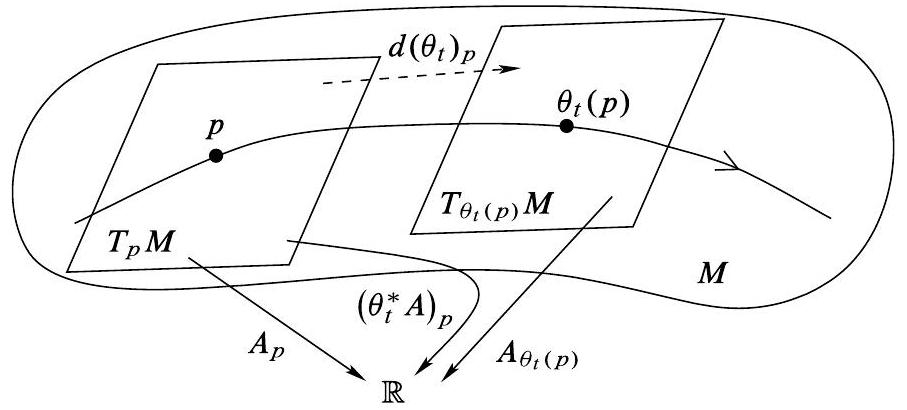
\includegraphics[max width=\textwidth, center]{2025_06_02_90020b9676379491a6e7g-340}
\end{itemize}

Fig. 12.1 The Lie derivative of a tensor field

Proposition 12.32. Let $M$ be a smooth manifold and let $V \in \mathfrak{X}(M)$. Suppose $f$ is a smooth real-valued function (regarded as a 0 -tensor field) on $M$, and $A, B$ are smooth covariant tensor fields on $M$.\\
(a) $\mathscr{L}_{V} f=V f$.\\
(b) $\mathscr{L}_{V}(f A)=\left(\mathscr{L}_{V} f\right) A+f \mathscr{L}_{V} A$.\\
(c) $\mathscr{L}_{V}(A \otimes B)=\left(\mathscr{L}_{V} A\right) \otimes B+A \otimes \mathscr{L}_{V} B$.\\
(d) If $X_{1}, \ldots, X_{k}$ are smooth vector fields and $A$ is a smooth $k$-tensor field,

$$
\begin{aligned}
\mathscr{L}_{V}\left(A\left(X_{1}, \ldots, X_{k}\right)\right)= & \left(\mathscr{L}_{V} A\right)\left(X_{1}, \ldots, X_{k}\right)+A\left(\mathscr{L}_{V} X_{1}, \ldots, X_{k}\right) \\
& +\cdots+A\left(X_{1}, \ldots, \mathscr{L}_{V} X_{k}\right)
\end{aligned}
$$

Proof. Let $\theta$ be the flow of $V$. For a real-valued function $f$, we can write

$$
\theta_{t}^{*} f(p)=f\left(\theta_{t}(p)\right)=f \circ \theta^{(p)}(t)
$$

Thus the definition of $\mathscr{L}_{V} f$ reduces to the ordinary derivative with respect to $t$ of the composite function $f \circ \theta^{(p)}$. Because $\theta^{(p)}$ is an integral curve of $V$, it follows from Proposition 3.24 that

$$
\left(\mathscr{L}_{V} f\right)(p)=\left.\frac{d}{d t}\right|_{t=0} f \circ \theta^{(p)}=d f_{p}\left(\theta^{(p)^{\prime}}(0)\right)=d f_{p}\left(V_{p}\right)=V f(p) .
$$

This proves (a).\\
The other assertions can be proved by the technique we used in Theorem 9.38: in a neighborhood of a regular point for $V$, if $\left(u^{i}\right)$ are coordinates in which $V=$ $\partial / \partial u^{1}$, then it follows immediately from the definition that $\mathscr{L}_{V}$ acts on a tensor field simply by taking the partial derivative of its coefficients with respect to $u^{1}$, and (b)(d) all follow from the ordinary product rule. The same relations hold on the support of $V$ by continuity, and on the complement of the support because the flow of $V$ is trivial there.

One consequence of this proposition is the following formula expressing the Lie derivative of any smooth covariant tensor field in terms of Lie brackets and ordinary directional derivatives of functions, which allows us to compute Lie derivatives without first determining the flow.

Corollary 12.33. If $V$ is a smooth vector field and $A$ is a smooth covariant $k$-tensor field, then for any smooth vector fields $X_{1}, \ldots, X_{k}$,

$$
\begin{aligned}
\left(\mathscr{L}_{V} A\right)\left(X_{1}, \ldots, X_{k}\right)= & V\left(A\left(X_{1}, \ldots, X_{k}\right)\right)-A\left(\left[V, X_{1}\right], X_{2}, \ldots, X_{k}\right) \\
& -\cdots-A\left(X_{1}, \ldots, X_{k-1},\left[V, X_{k}\right]\right)
\end{aligned}
$$

Proof. Just solve (12.9) for $\left(\mathscr{L}_{V} A\right)\left(X_{1}, \ldots, X_{k}\right)$, and replace $\mathscr{L}_{V} f$ by $V f$ and $\mathscr{L}_{V} X_{i}$ by $\left[V, X_{i}\right]$.

Corollary 12.34. If $f \in C^{\infty}(M)$, then $\mathscr{L}_{V}(d f)=d\left(\mathscr{L}_{V} f\right)$.\\
Proof. Using (12.10), for any $X \in \mathfrak{X}(M)$ we compute

$$
\begin{aligned}
\left(\mathscr{L}_{V} d f\right)(X) & =V(d f(X))-d f([V, X])=V X f-[V, X] f \\
& =V X f-(V X f-X V f)=X V f \\
& =d(V f)(X)=d\left(\mathscr{L}_{V} f\right)(X)
\end{aligned}
$$

One drawback of formula (12.10) is that in order to calculate what $\mathscr{L}_{V} A$ does to vectors $v_{1}, \ldots, v_{k}$ at a point $p \in M$, one must first extend them to vector fields in a neighborhood of $p$. But Proposition 12.32 and Corollary 12.34 lead to an easy method for computing Lie derivatives of smooth tensor fields in coordinates that avoids this problem, since any tensor field can be written locally as a linear combination of functions multiplied by tensor products of exact 1 -forms. The next example illustrates the technique.

Example 12.35. Suppose $A$ is an arbitrary smooth covariant 2 -tensor field, and $V$ is a smooth vector field. We compute the Lie derivative $\mathscr{L}_{V} A$ in smooth local coordinates $\left(x^{i}\right)$. First, we observe that $\mathscr{L}_{V} d x^{i}=d\left(\mathscr{L}_{V} x^{i}\right)=d\left(V x^{i}\right)=d V^{i}$. Therefore,

$$
\begin{aligned}
\mathscr{L}_{V} A & =\mathscr{L}_{V}\left(A_{i j} d x^{i} \otimes d x^{j}\right) \\
& =\mathscr{L}_{V}\left(A_{i j}\right) d x^{i} \otimes d x^{j}+A_{i j}\left(\mathscr{L}_{V} d x^{i}\right) \otimes d x^{j}+A_{i j} d x^{i} \otimes\left(\mathscr{L}_{V} d x^{j}\right) \\
& =V A_{i j} d x^{i} \otimes d x^{j}+A_{i j} d V^{i} \otimes d x^{j}+A_{i j} d x^{i} \otimes d V^{j} \\
& =\left(V A_{i j}+A_{k j} \frac{\partial V^{k}}{\partial x^{i}}+A_{i k} \frac{\partial V^{k}}{\partial x^{j}}\right) d x^{i} \otimes d x^{j}
\end{aligned}
$$

Recall that the Lie derivative of a vector field $W$ with respect to $V$ is zero if and only if $W$ is invariant under the flow of $V$ (see Theorem 9.42). It turns out that the Lie derivative of a covariant tensor field has exactly the same interpretation. If $A$ is a smooth tensor field on $M$ and $\theta$ is a flow on $M$, we say that $\boldsymbol{A}$ is invariant under $\boldsymbol{\theta}$ if for each $t$, the map $\theta_{t}$ pulls $A$ back to itself wherever it is defined; more precisely, this means

$$
d\left(\theta_{t}\right)_{p}^{*}\left(A_{\theta_{t}(p)}\right)=A_{p}
$$

for all ( $t, p$ ) in the domain of $\theta$. If $\theta$ is a global flow, this is equivalent to $\theta_{t}^{*} A=A$ for all $t \in \mathbb{R}$.

In order to prove the connection between Lie derivatives and invariance under flows, we need the following proposition, which shows how the Lie derivative can be used to compute $t$-derivatives at times other than $t=0$. It is a generalization to tensor fields of Proposition 9.41.

Proposition 12.36. Suppose $M$ is a smooth manifold with or without boundary and $V \in \mathfrak{X}(M)$. If $\partial M \neq \varnothing$, assume in addition that $V$ is tangent to $\partial M$. Let $\theta$ be the flow of $V$. For any smooth covariant tensor field $A$ and any ( $t_{0}, p$ ) in the domain of $\theta$,

$$
\left.\frac{d}{d t}\right|_{t=t_{0}}\left(\theta_{t}^{*} A\right)_{p}=\left(\theta_{t_{0}}^{*}\left(\mathscr{L}_{V} A\right)\right)_{p}
$$

Proof. After expanding the definitions of the pullbacks in (12.12), we see that we have to prove

$$
\left.\frac{d}{d t}\right|_{t=t_{0}} d\left(\theta_{t}\right)_{p}^{*}\left(A_{\theta_{t}(p)}\right)=d\left(\theta_{t_{0}}\right)_{p}^{*}\left(\left(\mathscr{L}_{V} A\right)_{\theta_{t_{0}}}(p)\right)
$$

Just as in the proof of Proposition 9.41, the change of variables $t=s+t_{0}$ yields

$$
\begin{aligned}
\left.\frac{d}{d t}\right|_{t=t_{0}} d\left(\theta_{t}\right)_{p}^{*}\left(A_{\theta_{t}(p)}\right) & =\left.\frac{d}{d s}\right|_{s=0} d\left(\theta_{s+t_{0}}\right)_{p}^{*}\left(A_{\theta_{s+t_{0}}}(p)\right) \\
& =\left.\frac{d}{d s}\right|_{s=0} d\left(\theta_{t_{0}}\right)_{p}^{*} d\left(\theta_{s}\right)_{\theta_{t_{0}}(p)}^{*}\left(A_{\theta_{s}\left(\theta_{t_{0}}(p)\right)}\right) \\
& =\left.d\left(\theta_{t_{0}}\right)_{p}^{*} \frac{d}{d s}\right|_{s=0} d\left(\theta_{s}\right)_{\theta_{t_{0}}(p)}^{*}\left(A_{\theta_{s}\left(\theta_{t_{0}}(p)\right)}\right) \\
& =d\left(\theta_{t_{0}}\right)_{p}^{*}\left(\left(\mathscr{L}_{V} A\right)_{\theta_{t_{0}}(p)}\right)
\end{aligned}
$$

Theorem 12.37. Let $M$ be a smooth manifold and let $V \in \mathfrak{X}(M)$. A smooth covariant tensor field $A$ is invariant under the flow of $V$ if and only if $\mathscr{L}_{V} A=0$.

\begin{itemize}
  \item Exercise 12.38. Prove Theorem 12.37.
\end{itemize}

\section*{Problems}
12-1. Give an example of finite-dimensional vector spaces $V$ and $W$ and a specific element $\alpha \in V \otimes W$ that cannot be expressed as $v \otimes w$ for $v \in V$ and $w \in W$.\\
12-2. For any finite-dimensional real vector space $V$, prove that there are canonical isomorphisms $\mathbb{R} \otimes V \cong V \cong V \otimes \mathbb{R}$.\\
12-3. Let $V$ and $W$ be finite-dimensional real vector spaces. Show that the tensor product space $V \otimes W$ is uniquely determined up to canonical isomorphism by its characteristic property (Proposition 12.7). More precisely, suppose $\tilde{\pi}: V \times W \rightarrow Z$ is a bilinear map into a vector space $Z$ with the following


\end{document}